\documentclass[12pt]{article}

% Only packages latex2html supports well
\usepackage{amsmath}
\usepackage{amssymb}
\usepackage{amsthm}
\usepackage{hyperref}
\usepackage{graphicx}

\title{%
  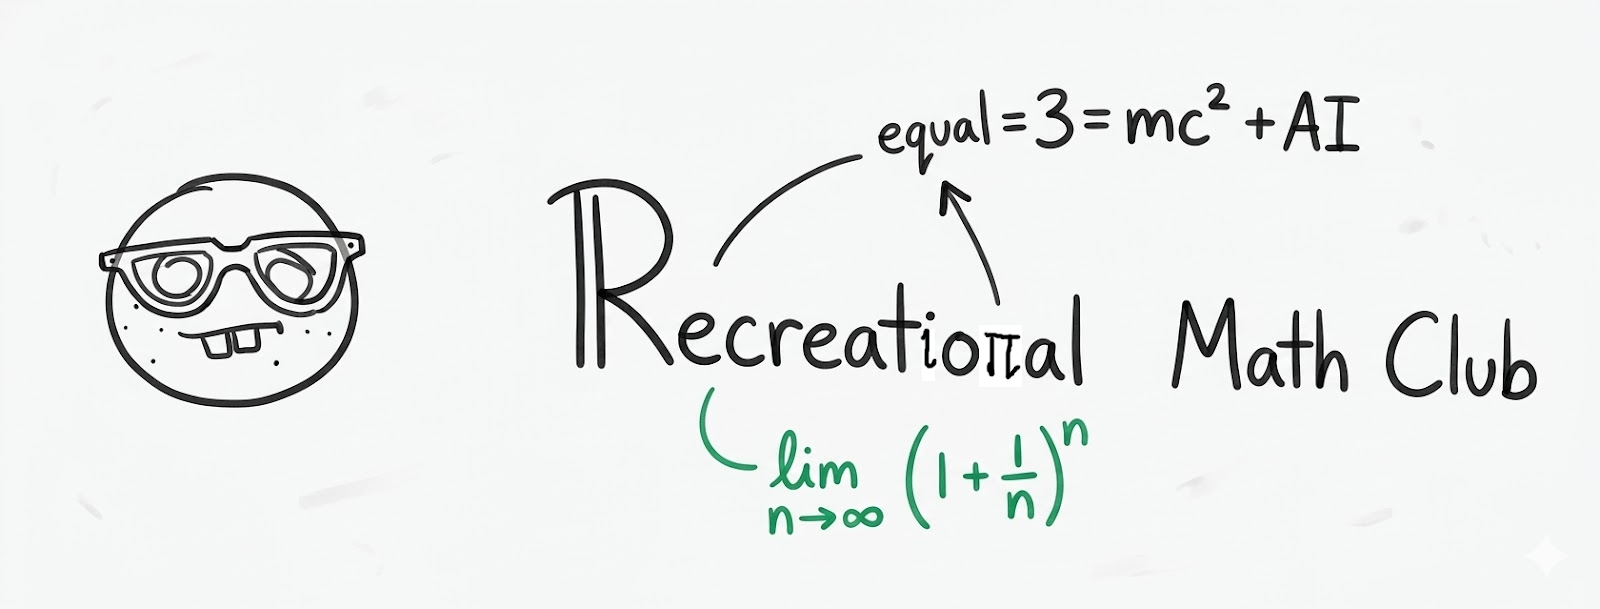
\includegraphics[width=0.8\linewidth]{img/logo.png} \\
  \large Indian Institute of Science, Bengaluru \\
} \\
\author{%
  {Dhairya Baxi \quad \texttt{baxivishal@iisc.ac.in}\\[2pt]
  Mahek Shamsukha \quad \texttt{maheks@iisc.ac.in}}
}
\date{Informal seminar series \quad$\cdot$\quad Fortnightly \quad$\cdot$\quad Est.\ 2024}

% Theorem environments
\theoremstyle{definition}
\newtheorem{defn}{Definition}[section]
\newtheorem{thm}[defn]{Theorem}
\newtheorem{prop}[defn]{Proposition}
\newtheorem{cor}[defn]{Corollary}
\newtheorem{lemma}[defn]{Lemma}
\newtheorem{example}[defn]{Example}

\theoremstyle{remark}
\newtheorem{remark}[defn]{Remark}
\newtheorem{moral}[defn]{Moral}

% Macros
\newcommand{\Z}{\mathbb{Z}}
\newcommand{\R}{\mathbb{R}}
\newcommand{\LP}{L_P}
\newcommand{\Ehr}{\operatorname{Ehr}}
\newcommand{\vol}{\operatorname{vol}}

\begin{document}
\maketitle
\tableofcontents

\begin{abstract}
The Recreational Mathematics Club is an informal seminar series at
IISc where students and faculty explore beautiful mathematics for its
own sake - no prerequisites, no pressure.
Talks span pure and applied topics, from elegant proofs to surprising
connections across fields.
We meet roughly every two weeks; everyone is welcome.
\[
  \lim_{n\to\infty}\!\left(1+\frac{1}{n}\right)^{\!n} = e
  \qquad
  \text{equal} = 3 = mc^2 + \mathrm{AI}
\]
\end{abstract}

%=================================================================
\section{Past Talks}

\begin{center}
\begin{tabular}{clll}
\hline
\textbf{\#} & \textbf{Title} & \textbf{Speaker(s)} & \textbf{Year} \\
\hline
2 & \textit{All about Lattices}              & {Mahek Shamsukha, \\ Dhairya Baxi} & 2025 \\
1 & \textit{Introduction to Ehrhart Theory} & Dhairya Baxi                    & 2024 \\
\hline
\end{tabular}
\end{center}

\begin{remark}
Talk notes from past sessions are available on request -
email the organizers.
\end{remark}

%=================================================================
\subsection{Talk 1: Introduction to Ehrhart Theory}

\subsubsection{Pick's Theorem}

\begin{defn}
A \emph{lattice polytope} $P \subset \R^d$ is a convex polytope
whose vertices all lie in $\Z^d$. Its \emph{lattice-point count} is
\[
  L_P(t) \;:=\; \#\bigl(tP \cap \Z^d\bigr), \qquad t \in \Z_{>0},
\]
where $tP = \{tx : x \in P\}$ is the $t$-th dilate.
\end{defn}

\begin{thm}[Pick, 1899]
Let $P \subset \R^2$ be a lattice polygon with $I$ interior lattice
points and $B$ boundary lattice points. Then
\[
  \operatorname{Area}(P) \;=\; I + \frac{B}{2} - 1.
\]
\end{thm}

For a lattice polygon the Ehrhart polynomial is
$L_P(t) = A\,t^2 + \tfrac{B}{2}\,t + 1$,
where $A = \operatorname{Area}(P)$.
Setting $t=1$ and applying Pick's theorem recovers $L_P(1) = I+B+1$.

\subsubsection{Reeve Tetrahedra: Pick Fails in 3-D}

\begin{defn}
For $r \geq 1$, the \emph{Reeve tetrahedron} $T_r$ has vertices
\[
  v_0=(0,0,0),\quad v_1=(1,0,0),\quad v_2=(0,1,0),\quad v_3=(1,1,r).
\]
\end{defn}

\begin{prop}
For every $r \geq 1$:
(i)~$I(T_r)=0$,\quad
(ii)~$B(T_r)=4$,\quad
(iii)~$\vol(T_r)=r/6$.
\end{prop}

\begin{moral}
The family $\{T_r\}$ shows that in dimension $\geq 3$ the data
$(I,B)$ alone does \emph{not} determine the volume. Pick's theorem
has no direct analogue in dimension $\geq 3$.
\end{moral}

The Ehrhart polynomial of the Reeve tetrahedra is
\[
  L_{T_r}(t) \;=\; \frac{r}{6}\,t^3 + t^2 + \frac{6-r}{6}\,t + 1.
\]

\subsubsection{Integer-Point Transforms and Brion's Theorem}

\begin{defn}
The \emph{integer-point transform} of $S \subset \R^d$ is
\[
  \sigma_S(\mathbf{z})
  \;:=\;
  \sum_{\mathbf{m}\,\in\, S\cap\Z^d} \mathbf{z}^{\mathbf{m}}.
\]
\end{defn}

\begin{thm}[Brion, 1988]
Let $P \subset \R^d$ be a rational polytope. Then, as rational
functions,
\[
  \sigma_P(\mathbf{z})
  \;=\;
  \sum_{v\;\text{vertex of }P} \sigma_{K_v}(\mathbf{z}),
\]
where $K_v$ is the vertex cone of $P$ at $v$.
\end{thm}

Each $\sigma_{K_v}$ is a rational function with poles at
$\mathbf{z}=\mathbf{1}$; summing over all vertices every pole
cancels, leaving the polynomial $\sigma_P$.

\subsubsection{Ehrhart's Theorem}

\begin{thm}[Ehrhart, 1962]
If $P$ is an integral convex $d$-polytope, then $L_P(t)$ is a
polynomial in $t$ of degree $d$.
\end{thm}

The \emph{Ehrhart series} is
\[
  \Ehr_P(z)
  \;:=\;
  1 + \sum_{t \geq 1} L_P(t)\,z^t
  \;=\;
  \frac{h^*(z)}{{(1-z)}^{d+1}},
\]
where $h^*(z)$ is a polynomial of degree $\leq d$ called the
\emph{$h^*$-polynomial} of $P$.

%=================================================================
\subsection{Talk 2: All about Lattices}

\subsubsection{Definitions}

\begin{defn}
A \emph{lattice} $\Lambda \subseteq \R^n$ is a discrete additive
subgroup. Equivalently, given linearly independent
$B=[b_1,\ldots,b_k]\in\R^{n\times k}$,
\[
  L(B) \;=\; \Bigl\{\sum_{i=1}^k x_i b_i : x_i\in\Z\Bigr\}
          \;=\; \{Bx : x\in\Z^k\}.
\]
Two bases generate the same lattice if and only if they are related
by a unimodular matrix ($\det = \pm 1$).
\end{defn}

\subsubsection{Fundamental Parallelepiped and Determinant}

\begin{defn}
The \emph{fundamental parallelepiped} of $L(B)$ is
\[
  \mathcal{P}(B)
  \;=\;
  \Bigl\{\sum_{i=1}^n x_i b_i : 0 \leq x_i < 1\Bigr\}.
\]
The \emph{determinant} is
$\det(L(B)) = \vol(\mathcal{P}(B)) = \prod_i \|b_i^*\|$,
where $b_i^*$ are the Gram-Schmidt vectors.
\end{defn}

\subsubsection{Minkowski's Theorem}

\begin{thm}[Minkowski]
Let $\Lambda$ be a lattice in $\R^n$ and $S$ a convex, centrally
symmetric body. If $\vol(S) > 2^n\det(\Lambda)$, then $S$ contains
a nonzero lattice point.
\end{thm}

\begin{thm}
If $p$ is prime with $p \equiv 1 \pmod{4}$, then
$p = a^2 + b^2$ for some $a,b\in\Z$.
\end{thm}

\begin{proof}[Proof sketch]
Since $p\equiv 1\pmod{4}$ there exists $i$ with $i^2\equiv-1\pmod p$.
Consider the lattice generated by $(1,0)^\top$ and $(i,p)^\top$
and apply Minkowski's theorem to the disc of radius $\sqrt{2p}$.
\end{proof}

\subsubsection{Hard Lattice Problems}

The following problems underlie modern lattice-based cryptography:

\begin{description}
  \item[SVP] Given a basis $B$, find a shortest nonzero vector in
    $L(B)$.
  \item[CVP] Given a basis $B$ and a target $\mathbf{t}$, find the
    closest lattice vector to $\mathbf{t}$.
  \item[SIVP] Find $n$ linearly independent vectors in $L(B)$, each
    as short as possible.
\end{description}

%=================================================================
\section{Suggested Topics}

A non-exhaustive list of areas members have expressed interest in.
Feel free to propose something entirely different.

\begin{itemize}
  \item \textbf{Combinatorics} - generating functions, bijective
        proofs, extremal problems
  \item \textbf{Number theory} - analytic, algebraic, or elementary
  \item \textbf{Topology} - knots, surfaces, fixed-point theorems
  \item \textbf{Discrete geometry} - polytopes, tilings, sphere
        packings
  \item \textbf{Probability} - random walks, percolation, paradoxes
  \item \textbf{Algebra} - representation theory, Galois theory
  \item \textbf{Analysis} - Fourier analysis, special functions,
        inequalities
  \item \textbf{Algorithms \& complexity} - lattice algorithms,
        cryptography
  \item \textbf{Mathematical physics} - integrable systems,
        statistical mechanics
\end{itemize}

%=================================================================
\section{How to Participate}

Anyone at IISc - students, postdocs, faculty - is welcome to
attend. Talks are informal and accessible. We encourage questions
mid-talk, tangents, and productive digressions.

\paragraph{Join the mailing list.}
Email either organizer (Section~\ref{sec:contact}) and ask to be
added.

%=================================================================
\section{Propose a Talk}

We welcome speakers from all backgrounds and career stages.
You need not be an expert - enthusiasm suffices.
Talks are typically 60-90 minutes including discussion.

\paragraph{How to propose.}
Send an email with subject \texttt{Talk proposal} (or similar) to
either organizer. Include a tentative title and a short description;
we will find a slot together.

%=================================================================
\section{Contact}
\label{sec:contact}

\begin{center}
\begin{tabular}{ll}
\hline
\textbf{Name} & \textbf{Email} \\
\hline
Dhairya Baxi (organizer) &
  \href{mailto:baxivishal@iisc.ac.in}{\texttt{baxivishal@iisc.ac.in}} \\
Mahek Shamsukha (organizer) &
  \href{mailto:maheks@iisc.ac.in}{\texttt{maheks@iisc.ac.in}} \\
\hline
\end{tabular}
\end{center}

\[
  \sum_{n=1}^{\infty}\frac{1}{n^2} \;=\; \frac{\pi^2}{6}
\]

\end{document}